\iflanguage{ngerman}
{\chapter{Grundlagen}}
{\chapter{Background}}
\label{sec:background}

% Vorstellung von mathematischem, technischem, algorithmischem oder anderem
% Grundlagenwissen, um die Arbeit zu verstehen

% Static/dynamic dataset?
% View dependent/independent exploded views?
% Wanted attributes of exploded views? 
% Short history of exploded views?
% Differences between exploded views in VR and 2D screens? 



When examining complex data sets or models, it is often important to understand the composition of the individual components and their order of assembly. 
This is especially the case for technical and biological models, where the order of composition defines the function. 
A problem that often arises is how to inspect the inner parts of such a model without breaking the compositional order. 
One possibility is to use filters and to cut away the frontal parts, but this is done at the expense of the overview and can make it difficult for the viewer to correctly identify the position of the part in the object. 
To avoid this, this work focuses on exploded views, as they offer the possibility to reveal internal parts of complex models while preserving their position in relation to other parts. 
Furthermore, they offer good interactive possibilities, which can also be transferred to the interaction in virtual reality.

Exploded views are drawings or information graphics that pull apart a complicated object as if it were blown up in a controlled manner. 
The individual parts are then spatially separated so that their position inside the object or model becomes visible. 
Often the projection of the object takes place in a planar view from the side or from slightly above.
This type of representation has a long history and can be found in many technical drawings, as the individual parts can be named and the order of assembly becomes clearly recognizable. %TODO add pictures

Looking at traditional hand-drawn explosion views, it becomes apparent that both the explosion direction in which the parts are moved and the spacing between the parts must be well chosen. 
In order to create the most informative explosion views, Li et al.\cite{Wilmot_Li_2008} describe five additional desirable conventions in their paper.
They can also be seen in figure \ref{fig:exampleExpl_Li2008}.
\begin{figure}[h]

	\centering
	%\vspace{-0.7cm}
	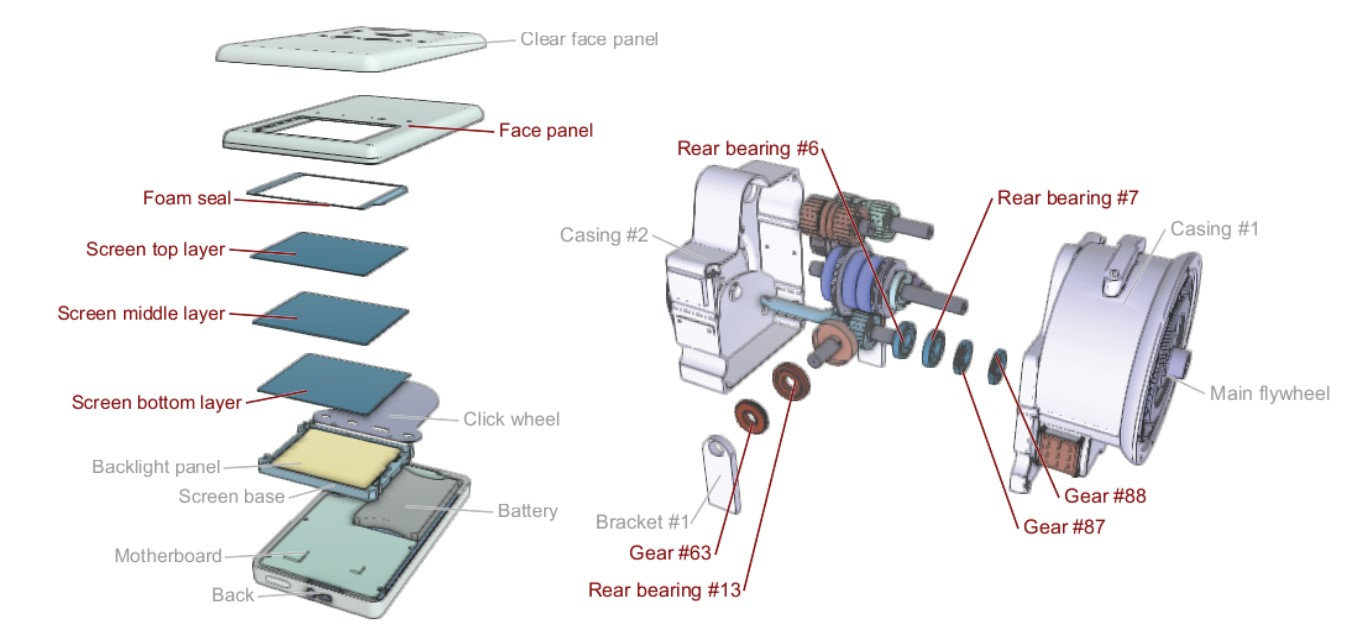
\includegraphics[width=.9\linewidth]{fig/Images/Li_2008}
	\caption[]{Exemplary exploded views generated with Li et al.'s system. On the left an exploded view of an iPod, on the right that of a transmission. Parts of interest are marked in red.[\cite{Wilmot_Li_2008}, Figure 10]}
	\label{fig:exampleExpl_Li2008}
\end{figure}


\begin{itemize}
	\item \textbf{Blocking constraints:} Parts should be translated so that they do not pass other parts, this is to show the viewer how the components fit together and indicate their relative position.
	\item \textbf{Visibility:} The spacing of all parts should be chosen so that each part of interest is visible.
	\item \textbf{Compactness:} Parts should be moved as little as possible from their original position to facilitate the viewer's mental reconstruction.
	\item \textbf{Canonical explosion directions:} Most objects have a canonical direction, i.e. an axis in which the object can best be aligned after the explosion. This is determined by various object-specific properties. In order to reduce the visual clutter, only a few of these axes should be chosen, otherwise the viewer will have difficulty recognizing the original composition.
	\item \textbf{Part hierarchy:} Complex models are sometimes divided into different exploded views and axes, this can illustrate the composition of smaller parts of the object.
	\label{items:best_practise}
\end{itemize}

If internal parts of an object are completely enclosed, it is necessary to either remove or cut open the outer part. According to Li et al., it should be ensured that when the outer object is cut, the distance with which the outer parts are pulled apart is kept as minimal as possible, whilst still leaving the inner parts visible.\cite{Wilmot_Li_2008}
In such cases it is also common to hide the outer parts to reveal the inner composition as it can be seen in figure \ref{fig:Li_2008_containerSplit}.
\begin{figure}[h]
	\centering
	%\vspace{-0.7cm}
	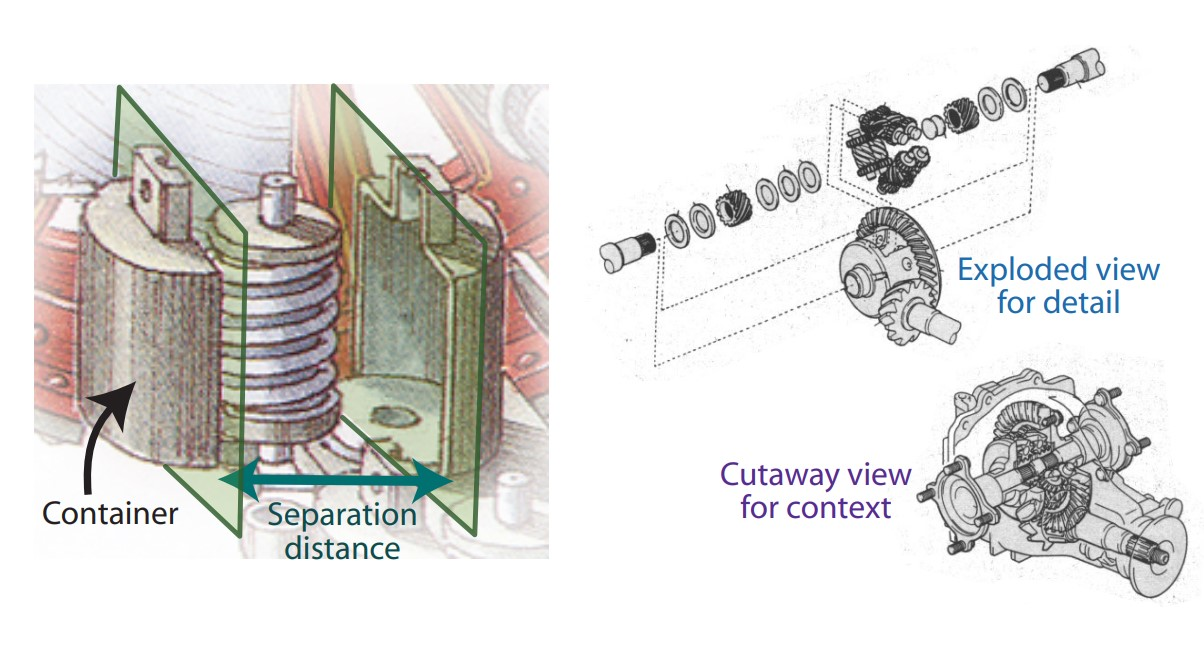
\includegraphics[width=.8\linewidth]{fig/Images/Li_2008_fig3}
	\caption[]{Ways to separate containers. The container is split on the left and shown as a contextual cutaway on the right.[\cite{Wilmot_Li_2008}, Figure 3]}
	\label{fig:Li_2008_containerSplit}
\end{figure}



A distinctive feature which is relevant for this work are the utilized data sets.
They represent the growth of an embryo, which begins with a few stem cells, which divide and reproduce over the course of the simulation. This creates new cells and cell populations.
They have been generated using the program \emph{Morpheus} which is being developed at the TU Dresden.\cite{morpheus_2022}
\emph{Morpheus} can be used to simulate and visualize the temporal changes of cell complexes and their evolution. 
The datasets thus represents a biological model in which there is no fixed order of composition and the individual parts may change their position and size over time.  
Figure \ref{fig:Dataset2D} shows a two-dimensional view of the data set at three time steps, which is created by Morpheus. Here it can be seen how the cell structure changes over time and how two populations form at a later time step. These are colored with blue and green. 
Figure \ref{fig:Dataset3D} shows a three-dimensional visualization of another dataset that was created with \emph{Morpheus}. This was created with ParaView\cite{paraview}.
\begin{figure}[h]
	\centering
	%\vspace{-0.7cm}
	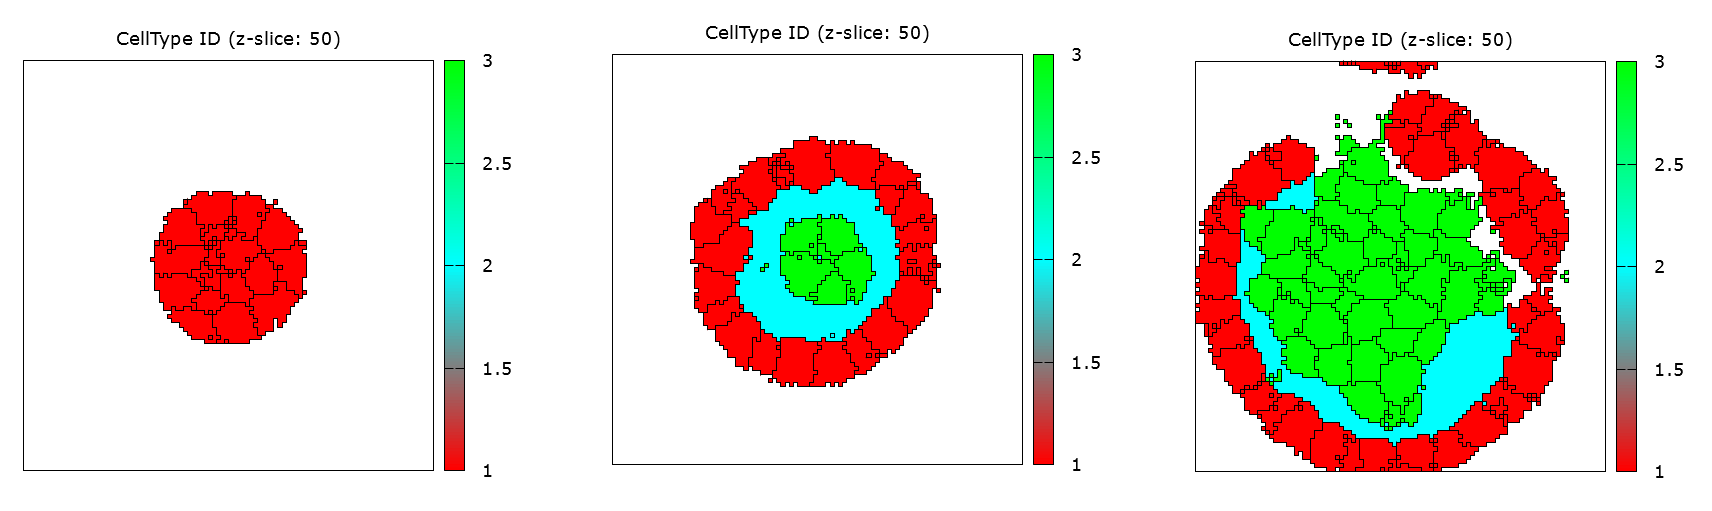
\includegraphics[width=1\linewidth]{fig/Images/Dataset2D}
	\caption[]{Two-dimensional data set visualization, which was created with \emph{Morpheus} at three different time steps $t$. Left: $t$=100, Middle: $t$=1500, Right: $t$=3000.}
	\label{fig:Dataset2D}
\end{figure}

\begin{figure}[h]
	\centering
	%\vspace{-0.7cm}
	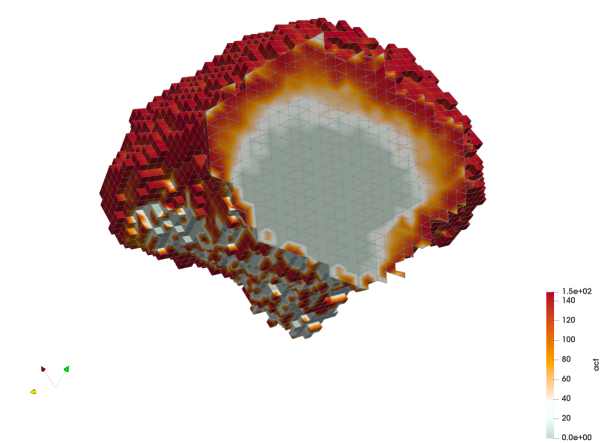
\includegraphics[width=0.7\linewidth]{fig/Images/Dataset3D}
	\caption[]{3D visualization of a Hapatocyte (liver cell) dataset which was simulated using Morpheus and created with ParaView.}
	\label{fig:Dataset3D}
\end{figure}
